\chapter{Κινητική θεωρία και εξισώσεις κατάστασης}
\label{apx:kinetic_theory}

\section{Γενικές έννοιες}
\label{apx:sec:general}
Σε αυτό το Κεφάλαιο θα δώσουμε συνοπτικά κάποιες βασικές έννοιες Θερμοδυναμικής και Στατιστικής Φυσικής που θα χρησιμοποιηθούν τόσο για την κλασική όσο και για την κβαντική περιγραφή των αερίων.

\textbf{1ος θερμοδυναμικός νόμος}: Το πρώτο θερµοδυναµικό αξίωµα µπορεί να διατυπωθεί ως εξής: "\textit{Η θερµότητα
είναι µια µορφή ενέργειας, και η ενέργεια διατηρείται}". Αν σε ένα αέριο προσθέσουµε θερµότητα, $\dbar Q$, τότε στη γενικότερη περίπτωση, θα αυξηθεί ταυτόχρονα και η εσωτερική του ενέργεια κατά $dU$ και θα µεταβληθεί ο όγκος του κατά $dV$ καταναλώνοντας ενέργεια $\dbar W = P dV$. Με άλλα λόγια, το ποσό θερμότητας που απορροφά ή αποβάλλεται από ένα θερμοδυναμικό σύστημα είναι ίσο με το αλγεβρικό άθροισμα της μεταβολής της εσωτερικής ενέργειας και του έργου που δαπανά ή παράγει το σύστημα.
Το πρώτο θερµοδυναµικό αξίωµα µε βάση τα παραπάνω µπορεί να περιγραφεί από την εξίσωση\footnote{Προσέξτε ότι τα $\dbar Q$ και $\dbar W$ είναι μη-τέλεια διαφορικά (inexact differentials). Αυτό σημαίνει ότι οι ποσότητες $Q,W$ δεν είναι καταστατικές συναρτήσεις αλλά εξαρτώνται από την διαδρομή (path functions) και άρα και τα διαφορικά τους εξαρτώνται και αυτά από τη διαδρομή.}
\begin{equation}
    \dbar Q = dU + \dbar W = dU + P dV
\end{equation}

\textbf{2ος θερμοδυναμικός νόμος}: Για μία αντιστρεπτή μεταβολή, η αλλαγή στην εντροπία ισούται με την αλλαγή στο ποσό θερμότητας δια την θερμοκρασία
\begin{equation}
    dS = \frac{\dbar Q}{T}
\end{equation}


\textbf{Εσωτερική ενέργεια}: Ονομάζεται το άθροισμα της ενέργειας όλων των ατόμων, μορίων και ιόντων ενός συστήματος. Η εσωτερική ενέργεια περιλαμβάνει πάντα τους παρακάτω όρους:
\begin{itemize}
    \item Κινητική ενέργεια λόγω της άτακτης κίνησης των σωματιδίων (γνωστή και ως θερμική κίνηση) --- translational energy
    \item Ενέργεια λόγω της περιστροφικής κίνησης των μορίων --- rotational energy
    \item Ενέργεια δόνησης των ατόμων στο μόριο --- vibrational energy
    \item Δυναμική ενέργεια λόγω των ελκτικών ή απωστικών δυνάμεων ανάμεσα στα άτομα, μόρια ή ιόντα του συστήματος --- potential energy
\end{itemize}

\textbf{Ιδανικό αέριο}: Ένα υποθετικό αέριο που αποτελείται από μη-διαχωρίσιμα σημειακά σωματίδια τα οποία συγκρούονται ελαστικά και για τα οποία οι διασωματιδιακές δυνάμεις μπορούν να αγνοηθούν. Ένα ιδανικό αέριο υπακούει στο \textbf{νόμο των ιδανικών αερίων}
\begin{equation}
    PV = NkT \Rightarrow P = \frac{\rho}{\mu m_H} kT
\end{equation}

Για το ιδανικό αέριο, θεωρούμε ότι τα σωματίδια που το αποτελούν δεν έχουν εσωτερική δομή, άρα εσωτερικοί μηχανισμοί όπως η δόνηση και η περιστροφή δεν συνεισφέρουν στην εσωτερική ενέργεια. Επίσης, η ενέργεια του σωματιδίου δεν εξαρτάται από τη θέση του, άρα δεν υπάρχει και συνεισφορά από "συντεταγμένες". Αυτό μας αφήνει μόνο με την κινητική ενέργεια. Δηλαδή, για ένα ιδανικό αέριο, η εσωτερική του ενέργεια ισούται με την κινητική ενέργεια και χαρακτηρίζεται πλήρως από αυτήν.
\begin{equation}
    \langle U \rangle = \langle E_{\text{kin}} \rangle = \frac{3}{2} NkT
\end{equation}
όπου $N$ ο αριθμός των σωματιδίων.

Στις τρεις διαστάσεις, υπάρχουν 3 ανεξάρτητες διευθύνσεις για την ορμή: $p_x, p_y, p_z$. Σύμφωνα με το θεώρημα της ισοκατανομής (equipartition theorem) η μέση ενέργεια ανά σωματίδιο
\begin{equation}
    \frac{\langle U \rangle}{N} = \frac{3}{2}kT
\end{equation}
μοιράζεται ισόποσα σε κάθε βαθμό ελευθερίας, ώστε σε κάθε διεύθυνση να αντιστοιχεί $\frac{1}{2}kT$

\textbf{Αδιαβατικές διεργασίες}: Συχνά ερχόμαστε αντιμέτωποι με διεργασίες οι οποίες συμβαίνουν σε τόσο σύντομο χρονικό διάστημα (π.χ. σε δυναμικό χρόνο) ώστε δεν υπάρχει ανταλλαγή θερμότητας με το περιβάλλον ($\dbar Q = dS = 0$). Αυτές οι διεργασίες ονομάζοναι "αδιαβατικές" και υπακούουν σε μία σχέση της μορφής
\begin{equation}
    P \propto \rho^{\gamma} 
\end{equation}
όπου το $\gamma$ ονομάζεται "αδιαβατικός δείκτης" (adiabatic index) 
\begin{equation}
    \gamma = \frac{q+5}{q+3}
\end{equation}
όπου $q$ ο αριθμός των εσωτερικών βαθμών ελευθερίας (για ιδανικό αέριο που τα σωματίδια είναι σημειακά έχουμε $q = 0 \rightarrow \gamma = 5/3)$.

\textbf{Θερμοδυναμική ισορροπία}: Ένα σύστημα λέγεται ότι βρίσκεται σε κατάσταση θερμοδυναμικής ισορροπίας όταν βρίσκεται σε
\begin{itemize}
    \item \textbf{μηχανική ισορροπία}: το διανυσματικό άθροισμα όλων των εξωτερικών και εσωτερικών δυνάμεων είναι μηδέν.
    \item \textbf{θερμική ισορροπία}: ένα σύστημα είναι σε θερμική ισορροπία με τον εαυτό του όταν δεν υπάρχουν θερμοβαθμίδες. Δύο συστήματα βρίσκονται σε θερμική ισορροπία μεταξύ τους όταν δεν υπάρχει μεταφορά θερμότητας. Για ένα αέριο συγκεκριμένης θερμοκρασίας που βρίσκεται σε θερμική ισορροπία, ισχύει η κατανομή Maxwell-Boltzmann για την κατανομή των ταχυτήτων των σωματιδίων που το αποτελούν.
    \item \textbf{χημική ισορροπία}: σε μια χημική αντίδραση, η κατάσταση χημικής ισορροπίας είναι αυτή κατά την οποία τόσο τα αντιδρώντα όσο και τα προϊόντα βρίσκονται σε συγκεντρώσεις που δεν υπάρχει η τάση για αλλαγή με τον χρόνο. Συνήθως αυτή η κατάσταση επέρχεται όταν ο ρυθμός παραγωγής των προϊόντων ισούται με τον ρυθμό της αντίστροφης διαδικασίας κατά την οποία τα προϊόντα σχηματίζουν ξανά τα αντιδρώντα από τα οποία προήλθαν.
    \item \textbf{στατιστική ισορροπία}: ένα σύστημα βρίσκεται σε κατάσταση στατιστικής ισορροπίας όταν ο πληθυσμός των ατόμων και των ιόντων που το αποτελούν δεν αλλάζει με τον χρόνο. Σε ένα τέτοιο σύστημα, ο πληθυσμός των καταστάσεων δίνεται από τον νόμο του Boltzmann.
\end{itemize}
Σε μία κατάσταση θερμοδυναμικής ισορροπίας, δεν υπάρχει ροή ενέργειας ή ύλης, δεν υπάρχουν αλλαγές φάσης ή δυναμικά που θα οδηγήσουν σε αλλαγές μέσα στο σύστημα. Ένα τέτοιο σύστημα δεν υπόκειται σε καμία αλλαγή όταν βρίσκεται απομονωμένο από το περιβάλλον του. Αν το σύστημα είναι απομονωμένο τόσο για την ύλη όσο και για την ακτινοβολία, και βρίσκεται σε κατάσταση μηχανικής ισορροπίας, τότε σταδιακά θα επέλθει σε κατάσταση θερμοδυναμικής ισορροπίας. Τέλος, για ένα σύστημα που βρίσκεται σε κατάσταση θερμοδυναμικής ισορροπίας, η θερμοκρασία ακτινοβολίας $T_R$, η θερμοκρασία λόγω της κινητικής ενέργειας των σωματιδίων $T$, καθώς και η θερμοκρασία διέγερσης $T_{\text{ex}}$ είναι ίσες μεταξύ τους.

\textbf{Τοπική θερμοδυναμική ισορροπία}: Πραγματική θερμοδυναμική ισορροπία είναι δύσκολο να επιτευχθεί (σχεδόν σε όλες τις περιπτώσεις ενέργεια διαφεύγει από το σύστημα με τη μορφή ακτινοβολίας, δηλαδή το σύστημα ψύχεται), και συχνά υπάρχουν θερμοβαθμίδες. Παρόλα αυτά, σε πολλά συστήματα (π.χ. αστέρες, μεσοασαστρικό μέσο) μπορούμε να εφαρμόσουμε τοπική θερμοδυναμική ισορροπία, που σημαίνει ότι το σύστημα βρίσκεται σε θερμοδυναμική ισορροπία αλλά μόνο σε μια πολύ μικρή περιοχή ενδιαφέροντος. Σε ένα σύστημα που βρίσκεται σε κατάσταση τοπικής θερμοδυναμικής ισορροπίας, υπάρχουν βαθμίδες θερμοκρασίας, πυκνότητας, πίεσης κτλ, αλλά θα είναι αρκετά μικρές στο διάστημα που ορίζεται από τη μέση ελεύθερη διαδρομή ενός σωματιδίου του αερίου.
Το γεγονός ότι τα φωτόνια στο εσωτερικό του Ήλιου κάνουν πολλές χιλιάδες χρόνια να φτάσουν στην επιφάνεια και άρα είναι τοπικώς "παγιδευμένα" είναι αποτέλεσμα της κατάστασης τοπικής θερμοδυναμικής ισορροπίας που επικρατεί στο εσωτερικό του Ήλιου.

\subsection{Καταστατικές εξισώσεις αερίων}
Ως καταστατική εξίσωση εννοούμε μία θερμοδυναμική εξίσωση που περιγράφει την κατάσταση της ύλης υπό συγκεκριμένες φυσικές συνθήκες. Συνήθως είναι της μορφής $P = P(\rho, T)$. Πολλές φορές είναι χρήσιμο να γράψουμε την καταστατική εξίσωση σε διαφορική μορφή. Η διαφορική μορφή μπορεί να βρεθεί αν ξεκινήσουμε γράφοντας την καταστατική εξίσωση γενικά ως έναν εκθετικό νόμο (power law)
\begin{equation}
    P = \rho^{\chi_\rho} T^{\chi_T}
\end{equation}
και άρα το ολικό διαφορικό είναι
\begin{align}
    \nonumber dP &= \left( \frac{\partial P}{\partial \rho} \right)_T d\rho + \left( \frac{\partial P}{\partial T} \right)_\rho dT \Rightarrow \\\nonumber\\
    \nonumber &\Rightarrow dP = \chi_\rho T^{\chi_T} \rho^{\chi_\rho - 1} d\rho +  \chi_T \rho^{\chi_\rho} T^{\chi_T - 1} dT \Rightarrow \\\nonumber\\
    \nonumber &\Rightarrow dP = \underbrace{\rho^{\chi_\rho} T^{\chi_T}}_{P} \left(\chi_\rho \rho^{-1} d\rho + \chi_T T^{-1} dT \right) \Rightarrow \\\nonumber\\
    &\Rightarrow \boxed{\frac{dP}{P} = \chi_\rho \frac{d\rho}{\rho} + \chi_T \frac{dT}{T}}
\end{align}

Αντιπαραβάλοντας τις σχέσεις
\begin{align*}
    \label{apx:eq:differential_form_of_eos}
    dP &= \left( \frac{\partial P}{\partial \rho} \right)_T d\rho + \left( \frac{\partial P}{\partial T} \right)_\rho dT \\\\
    \frac{dP}{P} &= \chi_\rho \frac{d\rho}{\rho} + \chi_T \frac{dT}{T}
\end{align*}
βρίσκουμε ότι τα εκθετικά $\chi_\rho, \chi_T$ δίνονται από τις σχέσεις
\begin{align*}
    \chi_\rho &= \frac{\rho}{P} \left( \frac{\partial P}{\partial \rho} \right)_T \\\\
    \chi_T &= \frac{T}{P} \left( \frac{\partial P}{\partial T} \right)_\rho
\end{align*}

Μπορεί κανείς όμως να βρει μία ακόμα πιο κομψή έκφραση των παραπάνω εκθετών ως εξής:
\begin{align*}
     P &= \rho^{\chi_\rho} T^{\chi_T} \Rightarrow \log \,P = \log \,\left( \rho^{\chi_\rho} T^{\chi_T} \right) = \log \,\rho^{\chi_\rho} + \log \,T^{\chi_T} \Rightarrow \\\\
     &\Rightarrow \log \,P = \chi_\rho \log \,\rho + \chi_T \log \,T
\end{align*}
Το ολικό διαφορικό άρα είναι
\begin{equation*}
    d\log \,P = \left( \frac{\partial \log \,P}{\partial \log \,\rho} \right)_T d \log \,\rho + \left( \frac{\partial \log \,P}{\partial \log \,T} \right)_\rho d \log \,T
\end{equation*}
ώστε
\begin{equation*}
    d \log \,P = \chi_\rho d\log \,\rho + \chi_T d \log \,T
\end{equation*}
και με αντιπαραβολή των δύο τελευταίων σχέσεων προκύπτει τελικά ότι
\begin{align}
    \chi_\rho &= \frac{\rho}{P} \left( \frac{\partial P}{\partial \rho} \right)_T = \left( \frac{\partial \log \,P}{\partial \log \,\rho} \right)_T \label{apx:eq:chi_rho}\\\nonumber\\
    \chi_T &= \frac{T}{P} \left( \frac{\partial P}{\partial T} \right)_\rho = \left( \frac{\partial \log \,P}{\partial \log \,T} \right)_\rho \label{apx:eq:chi_T}
\end{align}

Στην πιο γενική περίπτωση, τα $\chi_\rho, \chi_T$ εξαρτώνται και τα ίδια από τα $\rho, T$ αλλά αν είναι (προσεγγιστικά) σταθερά, η καταστατική εξίσωση γράφεται
\begin{equation}
    \label{apx:eq:eos_chi_rho_chi_T}
    P = P_0 \,\rho^{\chi_\rho} \,T^{\chi_T}
\end{equation}

Στην συνέχεια θα εξάγουμε την καταστατική εξίσωση για ένα τέλειο αέριο από τις αρχές της στατιστικής μηχανικής. Έστω $n(p)$ η κατανομή των ορμών των σωματιδίων του αερίου, δηλαδή με άλλα λόγια, το $n(p)dp$ αναπαριστά τον αριθμό των σωματιδίων ανά μονάδα όγκου που έχουν ορμή $p \in [p, p+dp]$. Αν η $n(p)$ είναι γνωστή, τότε η αριθμητική πυκνότητα, η πυκνότητα (εσωτερικής) ενέργειας, και η πίεση θα δίνονται από τα ακόλουθα ολοκληρώματα:
\begin{align}
    n &= \int_{0}^{\infty} n(p) dp \label{apx:eq:number_density_integral} \\\nonumber\\
    u &= \int_{0}^{\infty} E_{\text{kin}} n(p) dp = n \langle E_{\text{kin}} \rangle \label{apx:eq:energy_density_integral} \\\nonumber\\
    P &= \frac{1}{3}\int_{0}^{\infty} p \,v_p \,n(p) dp = \frac{1}{3} n \langle p \,v_p \rangle \label{apx:eq:pressure_integral} 
\end{align}
όπου $E_{\text{kin}}$ η κινητική ενέργεια σωματιδίου με ορμή $p$ και ταχύτητα $v_p$. Η σχέση \eqref{apx:eq:number_density_integral} είναι τετριμμένη ενώ η σχέση \eqref{apx:eq:energy_density_integral} προκύπτει από τον ορισμό του ιδανικού αερίου. Όμως η σχέση \eqref{apx:eq:pressure_integral} χρειάζεται εξήγηση.

\begin{figure}[h]
    \centering
    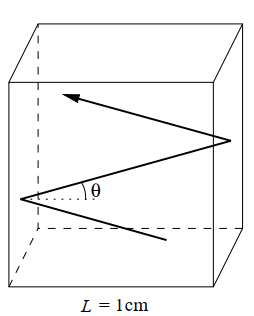
\includegraphics[scale = 0.6]{Figures/elastic_collision_in_a_box.png}
    \caption{Σωματίδιο αερίου μέσα σε ένα κυβικό κουτί όγκου $1 \,\text{cm}^3$. Κάθε σύγκρουση με τα τοιχώματα του κουτιού οδηγεί σε μεταφορά ορμής. Η πίεση μέσα στο κουτί είναι το αποτέλεσμα της συνολικής μεταφοράς ορμής από όλα τα σωματίδια μέσα στο κουτί.}
    \label{apx:fig:elastic_collisions}
\end{figure}

Ας υποθέσουμε ένα αέριο που αποτελείται από $N$ σωματίδια και το οποίο περιέχεται σε κυβικό κουτί με μήκος πλευρών $L = 1 \,\text{cm}$. Κάθε σωματίδιο ανακλάται από τα τοιχώματα του κουτιού και η πίεση στην συγκεκριμένη επιφάνεια είναι το αποτέλεσμα της μεταφοράς της ορμής από όλα τα σωματίδια που συγκρούονται με αυτή. Έστω ένα σωματίδιο με ορμή $p$ και αντίστοιχη ταχύτητα $v_p$ το οποίο πλησιάζει την μία πλευρά του κουτιού υπο γωνία $\theta$, όπως φαίνεται στο σχήμα \ref{apx:fig:elastic_collisions}. Ο χρόνος μεταξύ δύο συγκρούσεων στην ίδια επιφάνεια του κουτιού είναι
\begin{equation*}
    \Delta t = \frac{2L}{v_p \cos \,\theta} = \frac{2}{v_p \cos \,\theta}
\end{equation*}
Επειδή οι συγκρούσεις είναι ελαστικές ($p_f = - p_i$) η μεταφορά ορμής είναι διπλάσια από τη συνιστώσα της ορμής που είναι κάθετη στην επιφάνεια
\begin{equation*}
    \Delta p = p_f - p_i = 2p \cos \,\theta
\end{equation*}
'Αρα, ο ρυθμός με τον οποίο μεταφέρεται ορμή ανά σωματίδιο είναι
\begin{equation*}
    \frac{\Delta p}{\Delta t} = p \,v_p \,\cos^2 \,\theta
\end{equation*}
Ο αριθμός των σωματιδίων με $p \in [p,p+dp]$ και $\theta \in [\theta, \theta+d\theta]$ συμβολίζεται με $n(p, \theta) dp \,d\theta$. Η συνεισφορά αυτών των σωματιδίων στην πίεση τότε είναι
\begin{equation*}
    dP =  p \,v_p \,\cos^2 \,\theta \,n(p, \theta) dp \,d\theta
\end{equation*}
Επειδή οι ορμές είναι κατανεμημένες ισοτροπικά σε όλες τις διευθύνσεις μέσα σε μια στερεά γωνία $2\pi$, και η στερεά γωνία $d\omega$ που αντιστοιχεί σε αυτά τα σωματίδια με $\theta \in [\theta, \theta+d\theta]$ ισούται με $2\pi \sin \,\theta \,d\theta$ έχουμε ότι $n(p, \theta) = n(p) \sin \,\theta \,d\theta$ και άρα
\begin{equation*}
    dP = p v_p \cos^2 \,\theta \,n(p) \sin \,\theta \,d\theta \,dp
\end{equation*}
Η συνολική πίεση βρίσκεται με ολοκλήρωση σε όλες τις γωνίες ($0 \leq \theta \leq \pi/2$) και ορμές ώστε
\begin{align*}
    P &= \int_{0}^{\frac{\pi}{2}} \int_{0}^{\infty} p v_p \cos^2 \,\theta \,n(p) \sin \,\theta \,d\theta \,dp = \\\\
    &=\int_{0}^{\frac{\pi}{2}} \cos^2 \,\theta \,\sin \,\theta \,d\theta \int_{0}^{\infty} p v_p n(p) dp = \\\\
    &= \int_{0}^{1} \cos^2 \,\theta \, d(\cos \,\theta) \int_{0}^{\infty} p v_p n(p) dp \Rightarrow \\\\
    &\Rightarrow P = \frac{1}{3} \int_{0}^{\infty} p v_p n(p) dp = \frac{1}{3} n \langle p v_p \rangle
\end{align*}

Έχοντας ξεκαθαρίσει τα παραπάνω, θέλουμε τώρα να βρούμε μία σχέση μεταξύ της πίεσης και της εσωτερικής ενέργειας. Σύμφωνα με την ειδική σχετικότητα, η ορμή και η ταχύτητα των σωματιδίων σχετίζονται με την ενέργειά τους σύμφωνα με τις σχέσεις:
\begin{equation}
    \epsilon^2 = p^2 c^2 + m^2 c^4
\end{equation}
\begin{align}
    \nonumber \frac{\partial}{\partial p} (\epsilon^2) &= \frac{\partial}{\partial p} (p^2 c^2 + m^2 c^4) \Rightarrow 2\epsilon \frac{\partial \epsilon}{\partial p} = 2p c^2 \Rightarrow \\\nonumber\\
    &\Rightarrow \frac{\partial \epsilon}{\partial p} \equiv v_p = \frac{pc^2}{\epsilon}
\end{align}
Χρησιμοποιώντας αυτές τις σχέσεις μπορούμε να βρούμε σχέσεις μεταξύ της πίεσης και της εσωτερικής ενέργειας ενός ιδανικού αερίου στο μη-σχετικιστικό (NR) όριο και στο εξαιρετικά σχετικιστικό (ER) όριο:

\begin{itemize}
    \item \textbf{NR όριο}: σε αυτή την περίπτωση οι ορμές είναι $p \ll mc$
    
    $$\epsilon^2 = p^2 c^2 + m^2 c^4 \Rightarrow \epsilon^2 = c^2 \left(p^2 + m^2c^2 \right)$$
    Επειδή ισχύει ότι $p \ll mc$, άρα $\epsilon \simeq mc^2$ και συνεπώς
    $$v_p = \frac{pc^2}{\epsilon} = \frac{p}{m}$$
    Η κινητική ενέργεια είναι όπως περιμένουμε $E_{\text{kin}} = \frac{p^2}{2m}$ οπότε $\langle p v_p \rangle = \langle \frac{p^2}{m} \rangle = 2 \langle E_{\text{kin}} \rangle $.
    
    Τελικά, από τις σχέσεις \eqref{apx:eq:energy_density_integral}, \eqref{apx:eq:pressure_integral}, προκύπτει
    \begin{equation}
        \label{apx:eq:pressure_internal_energy_relation_for_nr_case}
        \boxed{P = \frac{2}{3}u}
    \end{equation}
    
    \item \textbf{ER όριο}: σε αυτή την περίπτωση έχουμε $p \gg mc$
    
    Αυτό σημαίνει ότι $\epsilon = pc$ και άρα $v_p = c \longrightarrow \langle p v_p \rangle = \langle pc \rangle = \langle \epsilon \rangle$.
    
    Τελικά, από τις σχέσεις \eqref{apx:eq:energy_density_integral}, \eqref{apx:eq:pressure_integral}, προκύπτει
    \begin{equation}
        \label{apx:eq:pressure_internal_energy_relation_for_er_case}
        \boxed{P = \frac{1}{3}u}
    \end{equation}
\end{itemize}

Γενικά μπορούμε να γράψουμε ότι 
\begin{equation}
    P = \zeta n \langle E \rangle
\end{equation}
όπου $\zeta = 2/3$ ή $\zeta = 1/3$ για το μη-σχετικιστικό και το σχετικιστικό όριο αντίστοιχα. Αυτό έρχεται σε συμφωνία με την διαίσθησή μας καθώς θα περιμέναμε η πίεση που προέρχεται από την σύγκρουση (λόγω ταχυτήτων) σωματιδίων να είναι ανάλογη της πυκνότητας των σωματιδίων και της κινητικής τους ενέργειας
\begin{equation*}
    P \sim n mv^2 \sim n E_{\text{kin}}
\end{equation*}


\subsubsection{Το κλασικό ιδανικό αέριο}
Σε ένα ιδανικό αέριο η κατανομή των ορμών δίνεται από την κατανομή Maxwell-Boltzmann
\begin{equation}
    n(p) dp = \frac{n}{(2\pi m kT)^{3/2}} \exp\left(- \frac{p^2}{2mkT}\right) 4\pi p^2 dp
\end{equation}
με την οποία θα ασχοληθούμε εκτενώς παρακάτω. Θα αποδείξουμε τότε ότι $\langle E_{\text{kin}} \rangle = \frac{3}{2} kT $ και άρα σύμφωνα με τη σχέση \eqref{apx:eq:pressure_internal_energy_relation_for_nr_case} ισχύει ότι\textbf{ η καταστατική εξίσωση ενός ιδανικού αερίου είναι}
\begin{equation}
    \boxed{P_{\text{gas}} = \frac{2}{3}u = \frac{2}{3} n \langle E_{\text{kin}} \rangle = nkT = \frac{\rho}{\mu m_H}kT}
\end{equation}
που είναι ο γνωστός νόμος των ιδανικών αερίων. Αυτό το αποτέλεσμα προήλθε θεωρώντας μη-σχετικιστικά κλασικά σωματίδια αλλά μπορεί να δειχτεί ότι η ίδια σχέση ισχύει και για σχετικιστικά κλασικά σωματίδια.

Παρατηρούμε ότι ο νόμος των ιδανικών αερίων προκύπτει από τη σχέση \eqref{apx:eq:eos_chi_rho_chi_T} για $\chi_\rho = \chi_T = 1$


\subsubsection{Το αέριο φωτονίων}
Στο Κεφάλαιο \ref{ch:Chapter4}, αποδείξαμε ότι η πυκνότητα ενέργειας της ακτινοβολίας είναι
\begin{equation}
    u = \alpha T^4
\end{equation}
Επειδή το αέριο φωτονίων είναι εξ' ορισμού σχετικιστικό, χρησιμοποιούμε τη σχέση \eqref{apx:eq:pressure_internal_energy_relation_for_er_case} για να βρούμε την \textbf{καταστατική εξίσωση ενός αερίου φωτονίων}
\begin{equation}
    \boxed{P_{\text{rad}} = \frac{1}{3}u = \frac{1}{3} \alpha T^4}
\end{equation}

Παρατηρούμε ότι η καταστατική εξίωση ενός αερίου φωτονίων προκύπτει από τη σχέση \eqref{apx:eq:eos_chi_rho_chi_T} για $\chi_\rho = 0$ και $\chi_T = 4$.



\subsubsection{Το κβαντικό ιδανικό αέριο}
(εκφυλισμενο μη-σχετικιστικο αεριο φερμιονιων, εκφυλισμενο σχετικιστικο αεριο φερμιονιων)





\section{Νόμος του Boltzmann}
Εαν έχουμε έναν μεγάλο αριθμό ατόμων σε ένα ζεστό, πυκνό αέριο, τα άτομα αυτά συνεχώς θα συγκρούονται μεταξύ τους με αποτέλεσμα να διεγείρονται σε διάφορα πιθανά ενεργειακά επίπεδα. Η διέγερση λόγω συγκρούσεων θα ακολουθηθεί από την αποδιέγερση των ατόμων με εκπομπή ακτινοβολίας (σε χρονική κλίμακα της τάξης των νανοδευτερολέπτων). Αν η θερμοκρασία και η πίεση παραμείνουν σταθερά, θα υπάρχει κάποιου είδους δυναμικής ισορροπίας μεταξύ των διεγέρσεων από τις συγκρούσεις και τις αποδιεγέρσεις, οδηγώντας σε μια συγκεκριμένη κατανομή των ατόμων στα διάφορα ενεργειακά επίπεδα. Όσο χαμηλότερη είναι η θερμοκρασία, τόσο πιο γρήγορα θα μειώνεται ο πληθυσμός των ατόμων που καταλαμβάνουν υψηλές ενεργειακές στάθμες. Μόνο στις πολύ υψηλές θερμοκρασίες θα μπορούν οι υψηλές ενεργειακές στάθμες να καταλαμβάνονται από έναν σημαντικό αριθμό ατόμων. Η εξίσωση Boltzmann περιγράφει ποιά θα είναι η κατανομή των ατόμων ανάμεσα σε διάφορα ενεργειακά επίπεδα, ως συνάρτηση της ενέργειας και της θερμοκρασίας\footnote{Οι πληροφορίες αντλήθηκαν από \url{https://phys.libretexts.org/Bookshelves/Astronomy__Cosmology/Book\%3A_Stellar_Atmospheres_(Tatum)}}. 

Ας φανταστούμε ένα κουτί (σταθερός όγκος) το οποίο περιέχει N άτομα, το καθένα από τα οποία έχει m δυνατά ενεργειακά επίπεδα. Ας υποθέσουμε ότι υπάρχουν $ N_j$ άτομα στο ενεργειακό επίπεδο $ E_j$. Ο συνολικός αριμός N των ατόμων δίνεται από τη σχέση
\begin{equation}
    \label{eq:apx:total_number_of_atoms}
     N = \sum_{i=1}^{m} N_i
\end{equation}
όπου ο ακέραιος θετικός δείκτης i τρέχει από το 1 μέχρι το m, συμπεριλαμβάνοντας την τιμή j.

Η συνολική εσωτερική ενέργεια του συστήματος U θα δίνεται από τη σχέση
\begin{equation}
    \label{eq:apx:internal_energy}
     U = \sum_{i=1}^{m} N_i E_i
\end{equation}

Τώρα, πρέπει να βρούμε πόσοι τρόποι υπάρχουν να κατανείμουμε N άτομα έτσι ώστε να υπάρχουν $ N_1$ στο πρώτο ενεργειακό επίπεδο, $ N_2$ στο δεύτερο κ.ο.κ. Θα συμβολίσουμε αυτόν τον αριθμό με $ \Omega$. Στην στατιστική φυσική το μέγεθος αυτό ονομάζεται στατιστικό βάρος και είναι ο αριθμός των (τρόπων) μικροκαταστάσεων που αντιστοιχούν στην ίδια (ενεργεια) μακροκατάσταση.
\begin{equation}
    \label{eq:apx:statistical_weight}
     \Omega = \frac{N!}{N_1! N_2! N_3! \dots N_j! \dots N_m!} = \frac{N!}{\prod_{i=1}^{m}N_i!}
\end{equation}
Η σχέση αυτή δεν είναι προφανής, γι' αυτό θα επιχειρησούμε να τη δικαιολογήσουμε εν μέρει. Ο αριθμός των τρόπων που μπορούμε να διαλέξουμε $ N_1$ άτομα από ένα σύνολο N ατόμων ώστε να καταλάβουν το πρώτο ενεργειακό επίπεδο, θα δίνεται από τον διωνυμικό συντελεστή $ \Omega_1 = {N \choose N_1}$. Για κάθε έναν από αυτούς τους τρόπους, πρέπει να ξέρουμε με πόσους τρόπους μπορούν να διαμοιραστούν $ N_2$ άτομα από τα εναπομείναντα $ N - N_1$ τα οποία θα καταλαμβάνουν την δεύτερη ενεργειακή στοιβάδα, οι οποίοι είναι $ \Omega_2 = {N - N_1 \choose N_2}$. Άρα, ο αριθμός των τρόπων με τους οποίους μπορούμε να κατανείμουμε τα άτομα στις δύο πρώτες ενεργειακές στοιβάδες, είναι το γινόμενο 
\begin{align*}
     \Omega &= { N \choose N_1} { N - N_1 \choose N_2} =  \frac{N!}{N_1! (N-N_1)!} \frac{(N-N_1)!}{N_2! (N-N_1 -N_2)!} \\\\
    &=  \frac{N!}{N_1!} \frac{1}{N_2!(N_2! - N_2!)} = \frac{N!}{N_1!N_2!}
\end{align*}
Συνεχίζοντας αυτή τη λογική, καταλήγουμε στον πολυωνυμικό συντελεστή
$$ \Omega = \prod_{i=1}^{m} \Omega_i =  { N \choose N_1} { N - N_1 \choose N_2} \dots = \frac{N!}{N_1!N_2! \dots N_m!}$$
Ίσως ο παραπάνω συλλογισμός γίνεται πιο αντιληπτός αν έχουμε στο μυαλό μας πως ο διωνυμικός συντελεστής μας δίνει τον αριθμό των υπαρκτών τρόπων να χωρίσουμε τις ποσότητες $ N_1$ και $ N - N_1$ από ένα σύνολο $ N$, σε δύο διακριτές καταστάσεις (two distinct bins). Ο πολυωνυμικός συντελεστής αντίστοιχα μας δίνει τον αριθμό των υπαρκτών τρόπων να χωρίσουμε τις ποσότητες $ N_1, N_2, \dots , N_m$ από ένα σύνολο $ N$, σε $ N$ διακριτές καταστάσεις ($ N$ distinct bins).

Τώρα πρέπει να βρούμε τους πιο πιθανούς διαμερισμούς, δηλαδή τους πιο πιθανούς αριθμούς $ N_1, N_2, \dots , N_m$. Ο πιο πιθανός καταμερισμός θα είναι αυτός που μεγιστοποιεί το $ \Omega$ ως προς το κάθε $ N_j$, και που υπόκειται στους περιορισμούς των σχέσεων \eqref{eq:apx:total_number_of_atoms} και \eqref{eq:apx:internal_energy}. Η εύρεση ακροτάτων μιας συνάρτησης υπό περιορισμούς, μας οδηγεί στην χρήση των πολλαπλασιαστών Lagrange. Επειδή όμως ο χειρισμός του παραγοντικού ($ N!$) είναι δύσκολος στην ανάλυση, θα βρούμε το μέγιστο του λογαρίθμου $ \ln{\Omega}$, χωρίς καμία ποιοτική διαφορά στο αποτέλεσμα. Παίρνοντας τον λογάριθμο της σχέσης \eqref{eq:apx:statistical_weight}, προκύπτει ότι
\begin{equation}
    \label{eq:apx:log_statistical_weight}
     \ln{\Omega} = \ln{N!} - \ln{N_1!} - \ln{N_2!} - \dots
\end{equation}

Χρησιμοποιώντας τον τύπο του Stirling:
\begin{equation}
    \label{eq:apx:stirling_formula}
     \ln{X!} = X \ln{X} - X
\end{equation}
στη σχέση \eqref{eq:apx:log_statistical_weight}, προκύπτει ότι
\begin{align}
    \label{eq:apx:non_factorial_terms_multiplicity}
   \nonumber  \ln{\Omega} &=  N \ln{N} - \cancel{ N} - (N_1 \ln{N_1} - \cancel{ N_1}) - (N_2 \ln{N_2} - \cancel{ N_2}) - \dots \\\nonumber \\
   \nonumber &=  N \ln{ N} -  N_1 \ln{ N_1} -  N_2 \ln{  N_2} - \dots \\ \nonumber \\
   &=  N \ln{N} - \sum_{i=1}^{m} N_i \ln{N_i}
\end{align}

Τώρα μπορούμε να προχωρήσουμε με την εύρεση του μεγίστου της συνάρτησης \eqref{eq:apx:non_factorial_terms_multiplicity}, ως προς μία από τις μεταβλητές, για παράδειγμα την $ N_j$, με τρόπο τέτοιο ώστε να είναι συνεπής με τους περιορισμούς των σχέσεων \eqref{eq:apx:total_number_of_atoms} και \eqref{eq:apx:internal_energy}. Χρησιμοποιώντας την μέθοδο των πολλαπλασιαστών Lagrange, έχουμε ότι για τον πιθανό αριθμό κατάληψης (most probable occupation number) του j ενεργειακού επιπέδου, ισχύει η σχέση:

\begin{equation}
    \label{eq:apx:occupation_number_condition}
     \frac{\partial \ln{\omega}}{\partial N_j} = \lambda \frac{\partial N}{\partial N_j} + \mu \frac{\partial U}{\partial N_j}
\end{equation}
Αναπτύσοντας τους όρους έχουμε:
\begin{align*}
    \frac{\partial \ln{\Omega}}{\partial N_j} &= \frac{\partial}{\partial N_j} \left( -N_j \ln{N_j}\right) = -\cancelto{1}{\frac{\partial N_j}{\partial N_j}} \ln{N_j} - \cancelto{1}{N_j \frac{\partial \ln{N_j}}{\partial N_j}} = - \ln{N_j} - 1 \\\\
    \lambda \frac{\partial N}{\partial N_j} &= \lambda \frac{\partial}{\partial N_j} \left( \sum_{i=1}^{m} N_i \right) = \lambda \sum_{i=1}^{m} \frac{\partial N_i}{\partial N_j} = \lambda \\\\
    \mu \frac{\partial U}{\partial N_j} &= \mu \frac{\partial}{\partial N_j} \left( \sum_{i=1}^{m} N_i E_i \right) = \mu \sum_{i=1}^{m} \frac{\partial \left( N_i E_i \right)}{\partial N_j} = \mu \sum_{i=1}^{m} \left( \frac{\partial N_i}{\partial N_j} E_i + N_i \cancelto{0}{\frac{\partial E_i}{\partial N_j}} \right) \\  
    &= \mu \sum_{i=1}^{m} \frac{\partial N_i}{\partial N_j}E_i = \mu E_j
\end{align*}

Αντικαθιστώντας τα παραπάνω στην σχέση \eqref{eq:apx:occupation_number_condition}, προκύπτει
\begin{equation}
    \label{eq:apx:occupation_number}
    - \ln{N_j} - 1 = \lambda + \mu E_j \Rightarrow N_j = C e^{-\mu E_j}
\end{equation}

Το μόνο που μένει να κάνουμε, είναι να προσδιορίσουμε τους πολλαπλασιαστές Lagrange $\lambda$ (ή ισοδύναμα $C = e^{-\lambda - 1}$) και $\mu$. Πολλαπλασιάζοντας την σχέση \eqref{eq:apx:occupation_number} με $N_j$, ενώ ταυτόχρονα αλλάζοντας τον δείκτη από $j$ σε $i$ και παίρνοντας το άθροισμα, έχουμε
\begin{align}
    \label{eq:apx:final_form}
   \nonumber N_j \ln{N_j} &+ \lambda N_j + N_j \mu E_j + N_j = 0 \Rightarrow \\ \nonumber \\
    \nonumber \Rightarrow \sum_{i=1}^{m} N_i \ln{N_i} &+ \lambda \sum_{i=1}^{m} N_i + \mu \sum_{i=1}^{m} N_i E_i + \sum_{i=1}^{m} N_i = 0 \\\nonumber \\
     \nonumber = \sum_{i=1}^{m} N_i \ln{N_i} &+ \lambda N + \mu U + N = 0 \Rightarrow \\\nonumber \\
   \Rightarrow N \ln{N} &- \ln{\Omega} + \lambda N + \mu U + N = 0
\end{align}

όπου στο τελευταίο βήμα κάναμε χρήση της σχέσης \eqref{eq:apx:non_factorial_terms_multiplicity}. Από τη Θερμοδυναμική και τη Στατιστική Φυσική γνωρίζουμε οτι ισχύουν για την εντροπία τα εξής:
\begin{equation}
    \label{eq:apx:thermodynamics_2nd_law}
    dU = TdS - PdV \longrightarrow \left( \frac{\partial U}{\partial S} \right)_V = T \Rightarrow \left( \frac{\partial S}{\partial U} \right)_V = \frac{1}{T}
\end{equation}
\begin{equation}
    \label{eq:apx:multiplicity}
    S = k \ln{\Omega}
\end{equation}

Συνδυάζοντας τις σχέσεις \eqref{eq:apx:thermodynamics_2nd_law} και \eqref{eq:apx:multiplicity} με την \eqref{eq:apx:final_form}, προκύπτει ότι:
\begin{equation}
    \label{eq:apx:mu_value}
    \left( \frac{\partial S}{\partial U} \right)_V = k \mu \Rightarrow \mu = \frac{1}{kT}
\end{equation}

Τέλος, αθροίζοντας τους όρους της σχέσης \eqref{eq:apx:occupation_number}, βρίσκουμε τον δεύτερο πολλαπλασιαστή Lagrange:
\begin{equation}
    \label{eq:apx:lambda_value}
    \sum_{i=1}^{m} N_i = C \sum_{i=1}^{m} e^{-E_i/(kT)} \Rightarrow C = \frac{N}{\sum_{i=1}^{m} e^{-E_i/(kT)}}
\end{equation}
που μας οδηγεί στην έκφραση:
\begin{equation}
    \label{eq:apx:unweighted_boltzmann}
    \frac{N_j}{N} = \frac{e^{-E_j/(kT)}}{\sum_{i=1}^{m}e^{-E_i/(kT)}}
\end{equation}

Παρόλα αυτά, μας μένει να λάβουμε υπόψιν ένα ακόμα πράγμα. Τα περισσότερα ενεργειακά επίπεδα σε ένα άτομο είναι εκφυλισμένα, δηλαδή υπάρχουν πολλές καταστάσεις με την ίδια ενέργεια. Γι' αυτό το λογο, για να βρούμε τον πληθυσμό ενός επιπέδου, πρέπει να προσθέσουμε τους πληθυσμούς των επιμέρους καταστάσεων. Έτσι, η εξίσωση \eqref{eq:apx:unweighted_boltzmann} πρέπει να πολλαπλασιαστεί με το στατιστικό βάρος g του επιπέδου
\begin{equation}
    \label{eq:apx:boltmann_equation}
   \boxed{ \frac{N_j}{N} = \frac{g_j e^{-E_j/(kT)}}{\sum_{i=1}^{m} g_i e^{-E_i/(kT)}} = \frac{g_j}{Z}e^{-E_j/(kT)}}
\end{equation}

Η εξίσωση \eqref{eq:apx:boltmann_equation} είναι γνωστή ως \textit{εξίσωση Boltzmann} ή κατανομή Boltzmann και μας δίνει την πιθανότητα να βρούμε $N_j$ άτομα στο ενεργειακό επίπεδο j, με ενέργεια $E_j$. Ο όρος $Z = \sum_{i=1}^{m} g_i e^{-E_i/(kT)}$ ονομάζεται συνάρτηση επιμερισμού (partition function). Ο υπολογισμός της, αν και πολύπλοκος, είναι καταρχήν δυνατός, αφού από τη θεωρία και το πείραμα είναι γνωστά τόσο το στατιστικό βάρος $g_i$, όσο και η ενέργεια διέγερσης $E_i$, κάθε στάθμης.

Το στατιστικό βάρος ενός ενεργειακού επιπέδου ενός ατόμου με μηδενικό πυρηνικο σπιν είναι $2J+1$, όπου το $J$ συμβολίζει την ολική στροφορμή του ατόμου. Αν το πυρηνικό σπιν είναι $I$, το στατιστικό βάρος του επιπέδου θα είναι $(2I+1)(2J+1)$. Παρόλα αυτά, ο παράγοντας $2J+1$ εμφανίζεται τόσο στον αριθμητή όσο και σε κάθε όρο του παρονομαστή της σχέσης \eqref{eq:apx:boltmann_equation}, άρα μπορεί να εξαλειφθεί. Άρα, όταν δουλεύουμε με την κατανομή Boltzmann, στις περισσότερες περιπτώσεις δεν είναι απαραίτητο να ανησυχούμε για το αν το άτομο έχει κάποιο συγκεκριμένο πυρηνικό σπιν, και το στατιστικό βάρος του κάθε επιπέδου στην εξίσωση \eqref{eq:apx:boltmann_equation} μπορεί να θεωρηθεί ότι είναι $g_j = 2J+1$.

Στην εξίσωση \eqref{eq:apx:boltmann_equation} συγκρίναμε τον αριθμό των ατόμων στο ενεργειακό επίπεδο $j$ με τον αριθμό των ατόμων σε όλα τα υπόλοιπα επίπεδα. Μπορούμε το ίδιο εύκολα να συγκρίνουμε τον αριθμό των ατόμων στο επίπεδο $j$ με τον αριθμό των ατόμων στη βασική στάθμη $0$:

\begin{equation}
    \label{eq:apx:ground_state}
    \frac{N_j}{N_0} = \frac{g_j}{g_0} e^{-E_j/(kT)}
\end{equation}
ή ακόμα μπορούμε να συγκρίνουμε τους πληθυσμούς δύο οποιοδήποτε ενεργειακών επιπέδων $i,j \ \text{με} \ j>i$:
\begin{equation}
    \label{eq:apx:boltzmann_two_levels}
    \frac{N_j}{N_i} = \frac{g_j}{g_i} e^{- (E_j - E_i)/ (kT)} = \frac{g_j}{g_i} e^{-h\nu/(kT)}
\end{equation}

\section{Συνάρτηση επιμερισμού}
Σε κάποια συστήματα, η ολική ενέργεια μπορεί να αποτελείται από διάφορες πηγές ενέργειας. Ας αναλογιστούμε, ως παράδειγμα, το απλό διατομικό μόριο. Η ενέργειά του μπορεί να είναι το άθροισμα της ενέργειας διέγερσης (λόγω ηλεκτρονίων), ενέργεια δόνησης, κινητική ενέργεια λόγω περιστροφής, αλλά και ενέργειας λόγω μεταφοράς. Αν αυτές οι πηγές ενέργειας είναι ανεξάρτητες η μία από τις άλλες, η ολική ενέργεια θα είναι το άθροισμα αυτών των συνεισφορών:
\begin{equation}
    \label{eq:apx:total_energy_diatomic_molecule}
    E_{\rm tot} = E_{\rm tran} + E_{\rm el} + E_{\rm vib} + E_{\rm rot}
\end{equation}
Στην πράξη, για πραγματικά μόρια, αυτό είναι απλά μία πρώτη προσέγγιση --- στην πραγματικότητα, υπάρχει κάποια αλληλεπίδραση μεταξύ των διάφορων συνεισφορών στην ολική ενέργεια, αλλά η πρόθεσή μας εδώ δεν είναι να επικεντρωθούμε στις λεπτομέρειες της μοριακής δομής αλλά να επισημάνουμε ένα μικρό σημείο που αφορά τις συναρτήσεις επιμερισμού. Δεδομένου λοιπόν ότι οι διάφορες ενεργειακές συνεισφορές είναι ανεξάρτητες μεταξύ τους και δεν αλληλεπιδρούν σημαντικά, η ολική ενέργεια όπως είπαμε είναι το άθροισμα των επιμέρους ενεργειακών συνεισφορών. Η ολική κυματοσυνάρτηση σε αυτή την περίπτωση είναι το γινόμενο των τριών επιμέρους κυματοσυναρτήσεων
\begin{equation}
    \label{eq:apx:wavefunctions}
    \psi = \psi_{\rm el} \psi_{\rm vib} \psi_{rot}
\end{equation}
Οι ποσότητες $\psi_{\rm vib}$ και $ E_{\rm vib}$ ελιναι οι κυματοσυναρτήσεις και τα ενεργειακά επίπεδα για έναν απλό αρμονικό ταλαντωτή, ενώ $\psi_{rot}$ και $E_{\rm rot}$ είναι οι κυματοσυναρτήσεις και τα ενεργειακά επίπεδα ενός στερεού ρότορα. Είναι αντιληπτό ότι ένα μόριο δεν μπορεί να είναι ταυτόχρονα στερεός ρότορας και αρμονικός ταλατωτής, γι' αυτό οι εξισώσεις \eqref{eq:apx:total_energy_diatomic_molecule} και \eqref{eq:apx:wavefunctions} είναι απλά προσεγγιστικές. Παρόλα αυτά, σε γενικές γραμμές, οι ενεργειακές διαφορές μεταξύ ηλεκτρονιακών ενεργειακών επιπέδων είναι οι μεγαλύτερες, οι διαφορές μεταξύ επιπέδων δονήσεων είναι ενδιάμεσες, και οι διαφορές μεταξύ ενεργειακών επιπέδων λόγω περιστροφής είναι οι μικρότερες, έτσι ώστε αυτή η πρώτη προσέγγιση είναι μια καλή αρχή. Ενεργειακά επίπεδα λόγω μεταφορικής κίνησης είναι πρακτικά συνεχή και μπορούν να υπολογισθούν ως κινητική ενέργεια. Επικεντρώνοντας την προσοχή μας γύρω από το σημείο ενδιαφέροντος για αυτό το κεφάλαιο, κάθε όρος της συνάρτησης επιμερισμού είναι της μορφής $e^{-E/(kT)}$, και άρα αν η ολική ενέργεια είναι το άθροισμα των επιμέρους συνεισφορών, όπως δείχνει η εξίσωση \eqref{eq:apx:total_energy_diatomic_molecule}, τότε η ολική (εσωτερική) συνάρτηση επιμερισμού είναι το γινόμενο των συναρτήσεων επιμερισμού των διάφορων συνειφορών:
\begin{equation}
    \label{eq:apx:total_partition_function}
    u = u_{\rm el} u_{\rm vib} u_{\rm rot}
\end{equation}

Σε εισαγωγικά μαθήματα κβαντομηχανικής, διδασκόμαστε --χωρίς ίσως να ξέρουμε γιατί-- το παράδειγμα "σωματίδιο σε κουτί". Αυτό ήταν χρήσιμο και θα το χρειαστούμε σε ό,τι ακολουθεί. Ίσως ήταν καλύτερο να ονομαζόταν "κύματα σε κουτί" καθώς αύτο που αναλύουμε στο συγκεκριμένο παράδειγμα είναι οι κυματοσυναρτήσεις που περιγράφουν την κυματική φύση ενός σωματιδίου. Αν το σωματίδιο (και το αντίστοιχο κύμα του) είναι περιορισμένο σε ένα κουτί, οι κυματοσυναρτήσεις περιορίζονται σε συναρτήσεις που έχουν έναν ακέραιο αριθμό αντι-κόμβων (antinodes) ανάμεσα σε δύο τοίχους, και κατά συνέπεια τα ενεργειακά επίπεδα μπορούν να έχουν μόνο διακριτές τιμές ---ένα ακόμα παράδειγμα της μη-αποφυγής των διακριτών ενεργειακών επιπέδων που προκύπτουν από συνοριακούς περιορισμούς. Αν το κουτί είναι ένας κύβος με πλευρά $a$, τότε τα ενεργειακά επίπεδα δίνονται από:
\begin{equation}
    \label{eq:apx:discrete_energy_levels_box}
    E_{n_x n_y n_z} = \frac{h^2}{8ma^2} \left(n^2_x + n^2_y + n^2_z \right)
\end{equation}

Αν έχουμε πολλά σωματίδια μέσα στο κουτί, μπορεί να ενδιαφερόμαστε για το πως τα διάφορα σωματίδια είναι κατενεμημένα (διαμοιρασμένα) μεταξύ των ενεργειακών επιπέδων. Με άλλα λόγια, πρέπει να ξέρουμε τη συνάρτηση επιμερισμού, η οποία είναι απλά:
\begin{equation}
    \label{eq:apx:box_partition_function_discrete}
    \sum_{n_x=0}^\infty \sum_{n_y=0}^\infty \sum_{n_z=0}^\infty \exp \left[ - \frac{h^2 \left(n_x^2 + n_y^2 + n_z^2 \right)}{8ma^2kT} \right]
\end{equation}

Αν το κουτί είναι πολύ μεγάλο, τα ενεγειακά επίπεδα είναι πολύ κοντά μεταξύ τους και σχεδόν συνεχή (αν το κουτί είναι απείρων διαστάσεων, δεν υπάρχουν συνοριακοί περιορισμοί και γι' αυτό υπάρχει ένα συνεχές φάσμα δυνατών ενεργειών). Αν τα επίπεδα είναι σχεδόν συνεχή, μπορούμε να αντικαταστήσουμε τα αθροίσματα με ολοκληρώματα και να πάρουμε το μεταφορικό κομμάτι της συνάρτησης επιμερισμού (που οφείλεται σε κίνηση του κέντρου μάζας):
\begin{align}
    \label{eq:apx:box_partition_function_integrals}
    \nonumber Q &= \int_0^\infty \int_0^\infty \int_0^\infty \exp \left[ - \frac{h^2 \left( n_x^2 + n_y^2 + n_z^2 \right)}{8ma^2kT } \right] dn_x dn_y dn_z \nonumber \\ \nonumber \\
    &=\left[ \int_0^\infty \exp \left( - \frac{h^2 n^2}{8ma^2kT } \right) dn \right]^3 \nonumber \\ \nonumber \\
    &= \left(\frac{2 \pi mkT}{h^2} \right)^{\frac{3}{2}} V
\end{align}
όπου $V = a^3$ είναι ο όγκος του κουτιού και $Z=Qu$ είναι η συνολική συνάρτηση επιμερισμού που περιλαμβάνει και το μεταφορικό αλλά και το "εσωτερικό" κομμάτι.




\section{Κατανομή Maxwell-Boltzmann}
Όπως είδαμε, η κατανομή Boltzmann μας δείχνει ότι η πιθανότητα ένα σωματίδιο να βρεθεί σε μία ενεργειακή κατάσταση $E$, μειώνεται εκθετικά όσο η ενέργεια αυξάνει. Μαθηματικά, η κατανομή Boltzmann γράφεται
\begin{equation}
    f(E) = A e^{-E/(kT)}
\end{equation}

Εάν αυτή η κατανομή εφαρμοστεί σε μία διάσταση για την ταχύτητα ενός σωματιδίου σε ένα αέριο, τότε επειδή $E = mu_x^2/2$, προκύπτει ότι
\begin{equation}
    \label{eq:apx:non_normalized_maxwell}
    f(u_x) = A e^{-mu_x^2/(2kT)}
\end{equation}
Για να βρούμε τον συντελεστή κανονικοποίησης $A$, πρέπει να λάβουμε υπόψιν ότι η πιθανότητα να βρούμε ο σωματίδιο σε κάποια τιμή της ταχύτητας είναι ίση με τη μονάδα. Έτσι:
\begin{equation}
    \label{eq:apx:normalize_integral}
    \int_{- \infty}^{+ \infty} f(u_x) du_x = 1 \Rightarrow A \int_{- \infty}^{+ \infty} e^{-mu_x^2/(2kT)} du_x = 1
\end{equation}
Κάνοντας την αντικατάσταση 
$$x^2 = \frac{m u_x^2}{2kT} \Rightarrow x = \sqrt{\frac{m}{2kT}} u_x \longrightarrow dx = \sqrt{\frac{m}{2kT}} du_x$$
από τη σχέση \eqref{eq:apx:normalize_integral} προκύπτει ότι:
\begin{align}
    \label{eq:apx:normalization_coefficient}
    \nonumber & A \sqrt{\frac{2kT}{m}} \int_{- \infty}^{+ \infty} e^{-mu_x^2/(2kT)} \sqrt{\frac{m}{2kT}} du_x = 1 \Rightarrow  \\ \nonumber \\ \nonumber
    & A \sqrt{\frac{2kT}{m}} \underbrace{\int_{- \infty}^{+ \infty} \sqrt{\pi}{e^{-x^2} dx}}_{=\sqrt{\pi}} = 1 \\ \nonumber \\
    & A = \sqrt{\frac{m}{2\pi kT}}
\end{align}
ώστε η σχέση \eqref{eq:apx:non_normalized_maxwell} να γράφεται τελικά:
\begin{equation}
    \label{eq:apx:normalized_maxwell_x_direction}
    f(u_x) = \sqrt{\frac{m}{2\pi kT}} e^{-mu_x^2/(2kT)}
\end{equation}

Η σχέση \eqref{eq:apx:normalized_maxwell_x_direction} ονομάζεται γραμμική πυκνότητα πιθανότητας (εφόσον μιλάμε για μία διάσταση). 'Ετσι, η πιθανότητα $dp(u_x)$ του να έχει ένα σωματίδιο ταχύτητα κατά τον άξονα των $x$ μεταξύ των τιμών $u_x$ και $u_x+du_x$ είναι:
\begin{equation}
    \label{eq:apx:gauss_probability_x}
    dp(u_x) = \sqrt{\frac{m}{2\pi kT}} e^{-mu_x^2/(2kT)} du_x = f(u_x) du_x
\end{equation}

Παρατηρούμε ότι η συνάρτηση που δίνει τη γραμμική πυκνότητα πιθανότητας $f(u_x)$ είναι συνάρτηση κατανομής Gauss, η οποία έχει τη μορφή
\begin{equation}
    \label{eq:apx:gauss_formula}
    G = C e^{-b^2u^2}
\end{equation}
όπου ο συντελεστής κανονικοποίησης $C = \sqrt{\frac{m}{2\pi kT}}$ καθορίζει το ύψος της καμπύλης, ενώ ο παράγοντας $b^2 = m/(2kT)$ καθορίζει το εύρος της κατανομής. Η κατανομή είναι κεντραρισμένη γύρω από το σημείο $u_x = 0$ καθώς λόγω των τυχαίων κινήσεων, η μέση διανυσματική ταχύτητα είναι μηδέν.

Επειδή ο ολικός αριθμός των σωματιδίων $N$, παραμένει σταθερός το ποσοστό $dN_x/N$ (ή ισοδύναμα η αριθμητική πυκνότητα $n=N/V$) των σωματιδίων που έχουν ταχύτητες κατά τον άξονα των $x$ στο διάστημα μεταξύ $u_x$ και $u_x+du_x$, θα ισούται με την πιθανότητα που υπολογίσαμε στη σχέση \eqref{eq:apx:gauss_probability_x}. Επομένως, ο αριθμός των μορίων που έχουν ταχύτητες στο διάστημα $\left[u_x, u_x + du_x \right]$ θα είναι:
\begin{align}
    \label{eq:apx:number_density_x_axis}
    \nonumber dN_x &= N dp(u_x) \longrightarrow dn_x = n dp(u_x) \Rightarrow\\ \nonumber \\ 
     dn_x &= n \sqrt{\frac{m}{2\pi kT}} e^{-mu_x^2/(2kT)} du_x = n f(u_x) du_x
\end{align}

Είναι προφανές ότι οι αντίστοιχες σχέσεις που δίνουν την πιθανότητα και την αριθμητική πυκνότητα των σωματιδίων με ταχύτητες κατά τη διεύθυνση $y$ και $z$ στα διαστήματα $\left[u_y, u_y + du_y \right]$ και $\left[u_z, u_z + du_z \right]$ αντίστοιχα, βρίσκονται αν αντικαταστήσουμε το σύμβολο $x$ με τα σύμβολα $y$ και $z$.

Τις περισσότερες φορές όμως δεν ενδιαφερόμαστε για τον αριθμό των σωματιδίων με ορισμένες ταχύτητες ως προς κάποια συγκεκριμένη διεύθυνση, κυρίως μάλιστα όταν δεν υπάρχει προτιμητέα κατεύθυνση στον χώρο από τη φυσική ή τη γεωμετρία του προβλήματος που μελετούμε. Συνήθως μας ενδιαφέρει η πιθανότητα $dp(u)$ ή το ποσοστό των σωματιδίων $dn(u)/n$ με συνολική ταχύτητα μεταξύ των τιμών $u$ και $u+du$, η οποία ταχύτητα προφανώς συνδέεται με τις ταχύτητες $u_x, u_y$ και $u_z$ μέσω της σχέσης:
\begin{equation}
    \label{eq:apx:total_velocity}
    u^2 = u_x^2 + u_y^2 + u_z^2
\end{equation}
Η πιθανότητα αυτή μπορεί να υπολογιστεί από τις σχέσεις \eqref{eq:apx:gauss_probability_x}, \eqref{eq:apx:number_density_x_axis} και \eqref{eq:apx:total_velocity}, αν χρησιμοποιήσουμε την αρχή του μοριακού χάους, σύμφωνα με την οποία οι ταχύτητες (άρα και οι κατανομές) κατά τις τρεις διευθύνσεις $x,y,z$ είναι ανεξάρτητες μεταξύ τους. Τότε, σύμφωνα με την θεωρία των πιθανοτήτων, η κοινή συνάρτηση κατανομής $f(u_x, u_y, u_z) $ που δίνει την πιθανότητα $dp(u)$ του να έχει ένα σωματίδιο ταχύτητες στα διαστήματα $[u_x, u_x + du_x], [u_y, u_y + du_y], [u_z, u_z + du_z]$, ισούται με το γινόμενο των $f(u_x), f(u_y)$ και $f(u_z)$. Έτσι, στις 3 διαστάσεις η πυκνότητα πιθανότητας είναι:
\begin{equation}
    \label{eq:apx:common_gauss_distribution}
    f(\boldsymbol{u}) = f(u_x, u_y, u_z) = f(u_x)f(u_y)f(u_z)
\end{equation}
και επομένως η πιθανότητα $dp(u)$ δίνεται από τη σχέση:
$$dp(u) = dp(u_x,u_y,u_z) =$$
\begin{align}
    \label{eq:apx:total_gauss_probability}
  \nonumber &= \sqrt{\frac{m^3}{(2 \pi kT)^3}} \exp \left(- \frac{m(u_x^2 + u_y^2 + u_z^2)}{2kT} \right) du_x du_y du_z \Rightarrow \\ \nonumber \\
    &\Rightarrow dp(u) = \sqrt{\frac{m^3}{(2 \pi kT)^3}} e^{- mu^2/(2kT)} du_x du_y du_z
\end{align}
όπου το γινόμενο $dV(u) = du_x du_y du_z$ εκφράζει τον στοιχειώδη όγκο στον χώρο των ταχυτήτων. Η σχέση \eqref{eq:apx:total_gauss_probability} απλοποιείται σημαντικά αν, αντί για καρτεσιανές, χρησιμοποιήσουμε σφαιρικές συντεταγμένες. Στην περίπτωση αυτή, ορίζεται έναν σφαιρικό κέλυφος με "ακτίνα" $u$ και συνιστώσες που δίνονται από τους μετασχηματισμούς:
\begin{align*}
    u_x & = u \sin{\theta} \cos{\phi} \\
    u_y & = u \sin{\theta} \sin{\phi} \\
    u_z & = u \cos{\theta}
\end{align*}
ενώ ο στοιχειώδης όγκος στο χώρο των ταχυτήτων μετασχηματίζεται βάσει της σχέσης $$dV = du_x du_y du_z = \left[ \frac{\partial (u_x, u_y, u_z)}{\partial (u, \theta, \phi)} \right] du d\theta d\phi$$

Η Ιακωβιανή υπολογίζεται ως:
\begin{equation*}
\displaystyle 
    \begin{bmatrix}
      \frac{\partial u_x}{\partial u} & 
        \frac{\partial u_x}{\partial \theta} & 
        \frac{\partial u_x}{\partial \phi} \\[2ex] % <-- 1ex more space between rows of matrix
      \frac{\partial u_y}{\partial u} & 
        \frac{\partial u_y}{\partial \theta} & 
        \frac{\partial u_y}{\partial \phi} \\[2ex]
      \frac{\partial u_z}{\partial u} & 
        \frac{\partial u_z}{\partial \theta} & 
        \frac{\partial u_z}{\partial \phi}
\end{bmatrix}
= \dots = u^2 \sin{\theta}
\end{equation*}
και άρα ο στοιχειώδης όγκος στο χώρο των ταχυτήτων εκφρασμένος σε σφαιρικές συντενταγμένες είναι $dV = u^2 \sin{\theta} du d\theta d\phi$ και, επειδή δεν μας ενδιαφέρει η διεύθυνση της ταχύτητας των σωματιδίων, μπορούμε να ολοκληρώσουμε την πιθανότητα ως προς τις γωνίες κατεύθυνσης
$$\int_{0}^{2\pi} \int_{0}^{\pi} d\phi \sin{\theta} d\theta = 4 \pi$$

Έτσι τελικά το ποσοστό των σωματιδίων με ταχύτητες μεταξύ $u$ και $u+du$ \textit{ανεξαρτήτως διεύθυνσης} είναι:
\begin{equation}
    \label{eq:apx:maxwell_boltzmann_speed_distribution}
    \frac{dn(u)}{n} = f(u) du = 4\pi \left(\frac{m}{2\pi kT}\right)^{\frac{3}{2}} e^{-\frac{mu^2}{2kT}} u^2 du
\end{equation}
Η συνάρτηση $f(u)$ είναι η συνάρτηση κατανομής της πυκνότητας πιθανότητας (πιθανότητα ανά μονάδα ταχύτητας) των ταχυτήτων και ονομάζεται κατανομή Maxwell-Boltzmann. Στο σημείο αυτό πρέπει να αναφέρουμε ότι η συνάρτηση κατανομής 
$$ f(u) = \left(\frac{m}{2\pi kT}\right)^{\frac{3}{2}} e^{-\frac{mu^2}{2kT}} u^2 $$
που εμφανίζεται στη σχέση \eqref{eq:apx:maxwell_boltzmann_speed_distribution}, αναφέρεται στην κατανομή των \textbf{μέτρων} των ταχυτήτων (Maxwell-Boltzmann speed distribution) και όχι στην κατανομή των διανυσματικών ταχυτήτων (Maxwell-Boltzmann velocity distribution) που δίνεται από τη συνάρτηση κατανομής της σχέσης \eqref{eq:apx:common_gauss_distribution}:
$$f(\boldsymbol{u}) = \left(\frac{m}{2\pi kT}\right)^{\frac{3}{2}} e^{- mu^2/(2kT)}$$

Παρατηρώντας τις δύο εκφράσεις, βλέπουμε ότι η συνάρτηση κατανομής των διανυσματικών ταχυτήτων είναι Γκαουσιανής φύσης (ως το γινόμενο των τριών επιμέρους Γκαουσιανών για την κάθε συνιστώσα), ενώ η συνάρτηση κατανομής των μέτρων των ταχυτήτων είναι κατανομή $\chi^2$ (chi square distribution) ως γινόμενο του Γκαουσιανού όρου και του πολυωνυμικού όρου $u^2$. Αυτό έχει ως αποτέλεσμα η κατανομή των μέτρων των ταχυτήτων να παρουσιάζει μια ασυμμετρία προς μεγάλες ταχύτητες (right-skewed) όπως φαίνεται και στο σχήμα \ref{fig:MBD_distribution}. Επίσης, ενώ η κατανομή των διανυσματικών ταχυτήτων είναι κεντραρισμένη γύρω από το μηδέν, η κατανομή των μέτρων των ταχυτήτων ξεκινάει από το μηδέν λόγω του όρου $u^2$. Αυτό είναι λογικό καθώς δεν νοείται αρνητικό μέτρο της ταχύτητας.


\begin{figure}[h]
   \centering
\begin{subfigure}[h]{0.45\textwidth}
	\centering
   	 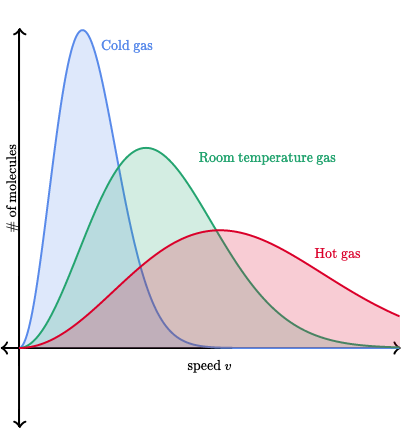
\includegraphics[width = \linewidth]{Figures/MBD_temperatures.png} 
\end{subfigure}
\begin{subfigure}[h]{0.54\textwidth}
	\centering
	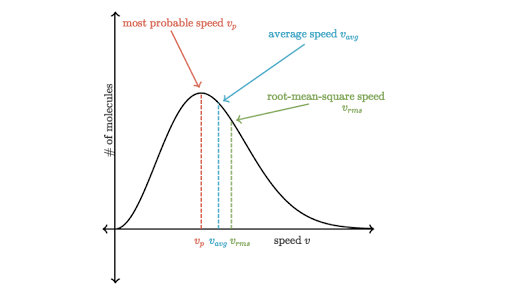
\includegraphics[scale=0.6]{Figures/MBD_velocities.png} 
    \end{subfigure}
    \caption{Κατανομή Maxwell-Boltzmann των μέτρων ταχυτήτων. Ο κάθετος άξονας εκφράζει τον αριθμό των σωματιδίων, αν και πολλές φορές επιλέγεται να δείχνει την πυκνότητα πιθανότητας αντ' αυτού η οποία είναι η πιθανότητα ανά μονάδα ταχύτητας να βρούμε ένα σωματίδιο με ταχύτητα κοντά στην $u$. \textbf{Left panel}: Εξάρτηση της κατανομής από τη θερμοκρασία. \textbf{Right Panel}: Ορισμός της πιο πιθανής ταχύτητας, της μέσης ταχύτητας, και της ταχύτητας $u_{\text{rms}}$.}
    \label{fig:MBD_distribution}
\end{figure}

Το ότι δεν υπάρχει προτιμητέα διεύθυνση στον χώρο και άρα η κατανομή των διανυσματικών ταχυτήτων ακολουθεί τη συμμετρική Γκαουσιανή κατανομή είναι εύκολα αντιληπτό. Γιατί όμως η συνάρτηση κατανομής των μέτρων των ταχυτήτων να είναι ασύμμετρη προς τα δεξιά, δηλαδή προς τις μεγάλες ταχύτητες; Η απάντηση είναι γιατί υπάρχουν πολλοί τρόποι να πάρουμε το μέτρο μιας μεγάλης ταχύτητας όταν συνυπολογίζουμε όλες τις κατευθύνσεις. Θα προσπαθήσουμε να το εξηγήσουμε δίνοντας ένα απλό παράδειγμα στον 2D χώρο:

Έστω δύο διανύσματα ταχύτητας $\boldsymbol{u_1}, \boldsymbol{u_2}$ με συνιστώσες $u_{1x}=1, u_{1y}=2$ και $u_{2x}=2, u_{2y}=1$ αντίστοιχα, ώστε:
\begin{align*}
    \boldsymbol{u_1} &= u_{1x} \hat{i} + u_{1y} \hat{j} = \hat{i} + 2 \hat{j} \\\\
    \boldsymbol{u_2} &= u_{2x} \hat{i} + u_{2y} \hat{j} = 2 \hat{i} +  \hat{j}
\end{align*}
Και τα δύο διανύσματα της ταχύτητας έχουν το ίδιο μέτρο: $$u_x = u_y = \sqrt{1^2 + 2^2} = \sqrt{2^2 + 1^2} = \sqrt{5}$$
Γενικεύοντας σε όλο το χώρο, γίνεται αντιληπτό ότι όσο μεγαλύτερο είναι το μέτρο της ταχύτητας, τόσο περισσότεροι συνδυασμοί των συνιστωσών $u_x, u_y, u_z$ (δηλαδή τόσο περισσότερα διανύσματα) υπάρχουν που θα δίνουν το ίδιο μέτρο. Άρα, ναι μεν όλες οι διευθύνσεις των ταχυτήτων είναι ισοπίθανες και άρα η συνάρτηση κατανομής τους θα είναι Γκαουσιανή, αλλά υπάρχουν περισσότερες καταστάσεις υψηλής ταχύτητας γεγονός που δίνει στην κατανομή την χαρακτηριστική ασυμμετρία προς τα δεξιά. 
Ο παράγοντας $4\pi u^2$ που υπάρχει στη σχέση \eqref{eq:apx:maxwell_boltzmann_speed_distribution}, λαμβάνει υπόψιν ακριβώς τη πυκνότητα καταστάσεων της ταχύτητας που είναι διαθέσιμη για τα σωματίδια.


\subsection{Χαρακτηριστικά και ιδιότητες}
Το ύψος (amplitude) της κατανομής Maxwell-Boltzmann δίνεται από τον συντελεστή κανονικοποίησης για τον οποίο γενικά ισχύει:
$$A \propto T^{-3/2}$$ 
Αντίστοιχα, για το εύρος της κατανομής ισχύει:
$$b^2 \propto T^{-1}$$
Άρα, υπό σταθερή μάζα, αν αυξάνεται η θερμοκρασία τότε ελλατώνεται το ύψος της καμπύλης ενώ παράλληλα φαρδαίνει όπως φαίνεται στο σχήμα \ref{fig:MBD_distribution}. Αυτό είναι λογικό καθώς το εμβαδόν κάτω από την καμπύλη της κατανομής μας δίνει τον συνολικό αριθμό των σωματιδίων. Έτσι, αν μειώσουμε τη θερμοκρασία του αερίου, η καμπύλη θα μετακινηθεί προς τα αριστερά και το ύψος θα αυξηθεί ώστε το εμβαδόν να παραμείνει σταθερό.

\subsubsection{Εύρεση πιθανότερης ταχύτητας}
Αν $u_p$ είναι η πιθανότερη ταχύτητα, τότε η καμπύλη παρουσιάζει μέγιστο στο $u_p$. Δηλαδή αρκεί
\begin{align*}
    u_p &= \frac{df(u)}{du} = 0 \Rightarrow \frac{d}{du} \left( A e^{-\frac{mu^2}{2kT}} u^2 \right) = 0 \\\\
    &\Rightarrow A \left[ \left( - \frac{mu}{kT} \right) e^{-\frac{mu^2}{2kT}} u^2 + 2u e^{-\frac{mu^2}{2kT}}  \right] = 0 \\\\
    &\Rightarrow 2u A e^{-\frac{mu^2}{2kT}} \left(1 - \frac{mu^2}{2kT} \right) = 0
\end{align*}
Η εξίσωση αυτή έχει τρεις λύσεις:
\begin{itemize}
    \item Αν $u=0$, τότε η κατανομή παρουσιάζει ελάχιστο.
    \item Αν $e^{-\frac{mu^2}{2kT}} = 0$, τότε $u \rightarrow \infty$ οπότε η κατανομή πάλι παρουσιάζει ελάχιστο.
    \item Αν $\frac{mu^2}{2kT} = 1$, τότε η κατανομή παρουσιάζει μέγιστο.
\end{itemize}
Έτσι, και σύμφωνα με το σχήμα \ref{fig:MBD_distribution}, η πιο πιθανή ταχύτητα είναι η 
\begin{equation}
    \label{eq:apx:most_probable_speed}
    \boxed{u_p = \sqrt{\frac{2kT}{m}}}
\end{equation}
και εκφράζει την πιο πιθανή τιμή της ταχύτητας που μπορεί να έχει ένα σωματίδιο στο αέριο.



\subsubsection{Στατιστικές ροπές}
Η συνάρτηση κατανομής Maxwell-Boltzmann περιέχει όλες τις πληροφορίες για τις στατιστικές ιδιότητες ενός τέλειου αερίου, δεν είναι όμως εύχρηστη επειδή ο υπολογισμός των πιθανοτήτων απαιτεί την ολοκλήρωση της σχέσης \eqref{eq:apx:maxwell_boltzmann_speed_distribution}, η οποία δεν είναι δυνατόν να γίνει αναλυτικά. Στην πράξη χρησιμοποιούμε συνήθως τις \textbf{στατιστικές ροπές} (moments) της σχέσης \eqref{eq:apx:maxwell_boltzmann_speed_distribution}, οι οποίες προκύπτουν πολλαπλασιάζοντας την συνάρτηση κατανομής επί της διάφορες δυνάμεις της ταχύτητας $u$ και ολοκληρώνοντας ως προς $u$. 
Η ροπή \textbf{μηδενικής τάξης} (μονοπολική/monopole) της σχέσης \eqref{eq:apx:maxwell_boltzmann_speed_distribution}

\begin{equation}
    \label{eq:apx:zeroth_order_moment}
    \int_{0}^{\infty} f(u) u^0 du = \int_{0}^{\infty} f(u) du = 1
\end{equation}
είναι εξ' ορισμού μονάδα, αφού παριστάνει την πιθανότητα του να έχει ένα σωματίδιο ταχύτητα $0 < u < \infty$, γεγονός που είναι προφανώς βέβαιο.
Η ροπή \textbf{πρώτης τάξης} (διπολική/dipole moment) μας δίνει, σύμφωνα με την θεωρία των πιθανοτήτων, τη \textbf{μέση ταχύτητα} $\langle u \rangle$ των σωματιδίων του αερίου
\begin{equation}
    \label{eq:apx:first_order_moment}
    \langle u \rangle = \int_{0}^{\infty} f(u) u du = A \int_{0}^{\infty} e^{-\frac{mu^2}{2kT}} u^3 du
\end{equation}
όπου $A = 4\pi \frac{m}{2\pi kT}^{3/2}$. Από πίνακες ολοκληρωμάτων γνωρίζουμε ότι $$\int_{0}^{\infty} x^3 e^{-ax^2} dx = \frac{1}{2a^2}$$
Χωρίς τη χρήση αυτού του τύπου, το ολοκλήρωμα της σχέσης \eqref{eq:apx:first_order_moment} λύνεται με την διαδοχική ολοκλήρωση κατά μέρη ως εξής:
\begin{align*}
    \langle u \rangle &= A \int_{0}^{\infty} e^{-\frac{mu^2}{2kT}} u^3 du = A \left( -\frac{kT}{m} \right) \int_{0}^{\infty} u^2 \underbrace{e^{-\frac{mu^2}{2kT}} d \left( -\frac{mu^2}{2kT} \right)}_{d\left(e^{- \frac{mu^2}{2kT}} \right)} = \\\\
   &= A \left( -\frac{kT}{m} \right) \int_{0}^{\infty} u^2 d\left(e^{- \frac{mu^2}{2kT}} \right) =  A \left( -\frac{kT}{m} \right) \left[ \cancelto{0}{\left. u^2 e^{-\frac{mu^2}{2kT}} \right|_{0}^{\infty}} - \right.\\\\
   &- \left. \int_{0}^{\infty} e^{-\frac{mu^2}{2kT}} 2u du \right] = 2A \left(\frac{kT}{m} \right) \int_{0}^{\infty} e^{-\frac{mu^2}{2kT}} u du = \\\\
   &= -2A \left(\frac{kT}{m} \right)^2 \int_{0}^{\infty} e^{-\frac{mu^2}{2kT}} d \left( -\frac{mu^2}{2kT} \right) = -2A \left(\frac{kT}{m} \right)^2 \int_{0}^{\infty} d\left(e^{- \frac{mu^2}{2kT}} \right) = \\\\
   &= -2A \left(\frac{kT}{m} \right)^2 \cancelto{-1}{\left[ e^{- \frac{mu^2}{2kT}} \right]_{0}^{\infty}} = 2A \left(\frac{kT}{m} \right)^2 
\end{align*}
Αντικαθιστώντας την τιμή της σταθεράς $A$ προκύπτει ότι η μέση ταχύτητα είναι
\begin{equation}
    \label{eq:apx:mean_speed}
     \boxed{\langle u \rangle = \sqrt{\frac{8kT}{\pi m}}}
\end{equation}
Από το σχήμα \ref{fig:MBD_distribution} φαίνεται ότι η μέση ταχύτητα βρίσκεται πιο δεξιά από την πιο πιθανή τιμή της ταχύτητας. Αυτό συμβαίνει γιατί η κατανομή παρουσιάζει μια "ουρά" προς τα δεξιά, η οποία "τραβάει" την μέση τιμή προς τα δεξιά της κορυφής. Με άλλα λόγια, υπάρχουν περισσότερες υψηλές από χαμηλές ταχύτητες.

Τέλος, η ροπή \textbf{δεύτερης τάξης} (τετραπολική ροπή/quadruple moment) μας δίνει τη \textbf{μέση τετραγωνική ταχύτητα} των σωματιδίων του αερίου
\begin{equation}
    \label{eq:apx:quadruple_moment}
    \langle u^2 \rangle = u_{\text{rms}} = \int_{0}^{\infty} f(u) u^2 du = A \int_{0}^{\infty} e^{-\frac{mu^2}{2kT}} u^4 du
\end{equation}
Η λύση του ολοκληρώματος έχει ως εξης:
\begin{align*}
    u_{\text{rms}} & = A \int_{0}^{\infty} e^{-\frac{mu^2}{2kT}} u^4 du = -A \left( \frac{kT}{m} \right) \int_{0}^{\infty} e^{-\frac{mu^2}{2kT}} u^3 d \left( - \frac{mu^2}{2kT} \right) = \\\\
    &= -A \left( \frac{kT}{m} \right) \int_{0}^{\infty} u^3 d \left( e^{- \frac{mu^2}{2kT}} \right) = -A \left( \frac{kT}{m} \right) \left [ \cancelto{0}{\left. u^3 e^{- \frac{mu^2}{2kT}} \right|_{0}^{\infty}} - \right. \\\\
    &- \left. 3 \int_{0}^{\infty} u^2 e^{-\frac{mu^2}{2kT}} du \right] = \frac{3kT}{m} \int_{0}^{\infty} A e^{-\frac{mu^2}{2kT}} u^2 du = \\\\
    &= \frac{3kT}{m} \cancelto{1}{\int_{0}^{\infty} f(u) du} = \frac{3kT}{m}
\end{align*}
Άρα, η μέση τετραγωνική ταχύτητα των σωματιδίων είναι
\begin{equation}
    \label{eq:apx:rms_speed}
    \boxed{u_{\text{rms}} = \frac{3kT}{m}}
\end{equation}

Από τη σχέση \eqref{eq:apx:rms_speed} προκύπτει και ότι η μέση κινητική ενέργεια των σωματιδίων ενός τέλειου αερίου δίνεται από τη σχέση
\begin{equation}
    \label{eq:apx:mean_kinetic_energy}
    \langle E \rangle = \frac{1}{2} m \langle u^2 \rangle = \frac{3}{2} kT
\end{equation}
που συνδέει την μέση κινητική ενέργεια με τη θερμοκρασία του αερίου.

Στο σημείο αυτό αξίζει να αναφέρουμε ότι η τιμή της συνάρτησης κατανομής Maxwell-Boltzmann πέφτει πολύ γρήγορα με την ταχύτητα. Έτσι συνήθως δεχόμαστε πως υπάρχει "αισθητή" αριθμητική πυκνότητα σωματιδίων μέχρι ταχύτητα ίση με $3 \sqrt{u_{\text{rms}}}$.